\section{Technical Description}
\label{sec:technical}

%%%%%%%%%%%%%%%%%%%%%%%%%%%%%%%%%%
%
% Alternate Solutions
%
%%%%%%%%%%%%%%%%%%%%%%%%%%%%%%%%%%

\subsection{Analysis of Alternate Solutions}

\subsubsection{Aircraft type}

The CONOPS for the competition initially lead to two potential types of aircraft,
a fixed-wing aircraft or a helicopter. A fixed wing would help in the ability
to travel long distances in an efficient manner, as well as design the airframe
to easily hold passengers. On the other hand, a fixed-wing aircraft will have
great difficulty take-off and landing within the limitations, since a runway
would be necessary.

Conversely, a helicopter has the ability to hover and take-off and land in more
constrained spaces with little difficulty. Helicopters also would be easier to
land near debris with higher precision, which can be important when taking into
consideration the weather during competition. However, helicopters require
significantly more skill to build. WARG as a team also has limited experience
working with helicopters, especially with much of the custom hardware and
software,such as ZeroPilot not being initially designed with helicopters in
mind.

Quadcopters were briefly considered, however ultimately proved to be
unfeasible. The requirements for long-range flight as well as the payload type,
a realistic flight cabin, seemed impractical, and reaching the desired flight
times with an aerodynamically unstable aircraft would only hurt efficiency.

The final decision was to move forward with a hybrid design of a fixed-wing
aircraft with a pusher motor and four extra vertical motors. The extra motors
are in a configuration similar to a quadcopter, which are only used during
vertical take-off and landing. This allows us to take best advantage of the
efficiency that is gained with a fixed wing aircraft and the lift it creates
while cruising, and meet the requiremets of landing in an urban environment as
required by the competition.

\todo{image of aircraft design here}

\subsubsection{Flight Control Software}

A major focus for this year's competition has been on the level of automation
that can be incorporated into completing task 1 and task 2. One of the most
versatile and popular flight software is ArduPilot. It provides more than
sufficient levels of configurability and flexibility, and has a capable
autopilot system that can be tweaked for almost any mission requirements, which
makes it a great option. Over the past few years, the embedded flight software
(EFS) team at WARG has been in development of a custom FreeRTOS based operating
system, and is instead the flight control software of choice.

Using a custom solution built from the ground up provides numerous advantages.
Primarily, using ZeroPilot gives more control and flexibility to implement
necessary features to specification. It provides the the aircraft further
control over each subsystem, and communication between different components,
such as the CV system and the ground station can be tweaked to a higher degree
of customisability. With this further level of customisability, the hope is
that the system as a whole has a reduced level of complexity.

\subsubsection{Motors, Propellers, and Batteries}

This year's competition provides teams more freedom and flexibility with the the
the design. There is a soft restriction placed of 5kg which provides the ability
to earn extra points in task 2.

\todo{Need to discuss how we compromised our weight (what is our current
target?) and how many passengers, and then include calculations we made for
motors, weight, and the batteries we picked.}

\todo{include image of calculations and flight time calculations}

\subsubsection{Computer Vision Systems}

\todo{Here are the list of items that need to be discussed here:}

\begin{itemize}
	\item What CV model and neural network type are we using?
	\item Why did we pick that over the alternatives?
	\item discuss our usage of the the jetson onboard 
	\item discuss increased level of complexity and possibility of things to
		go wrong if we instead did cv on the ground instead (losing
		connectivity, failure)
\end{itemize}

\subsubsection{Wireless/RF communication}

At the competition last year, substantial interference 

%%%%%%%%%%%%%%%%%%%%%%%%%%%%%%%%%%
%
% Solution Overview
%
%%%%%%%%%%%%%%%%%%%%%%%%%%%%%%%%%%

\subsection{Solution Overview}

%%%%%%%%%
% Reorganise sub sections for solutions + features
%%%%%%%%

\todo{diagram/chart of the full system outline}


%%%%%%%%%%%%%%%%%%%%%%%%%%%%%%%%%%
%
% Features and Capabilties
%
%%%%%%%%%%%%%%%%%%%%%%%%%%%%%%%%%%

\subsection{Features and Capabilities}

\subsubsection{ZeroPilot}

WARG's autopilot software comprises of 3 primary subcomponents controlled by
\textbf{System Manager} (SM). SM is a centralized unit for handling the state
of the system. It handles all inputs from sensors like the accelerometer and
gyroscope, outputs to motors and servos, the full flight state of the aircraft,
and deciding when other subcomponents run and integration between them.

\begin{figure}[h]
	\caption{State of SM}
	\centering
	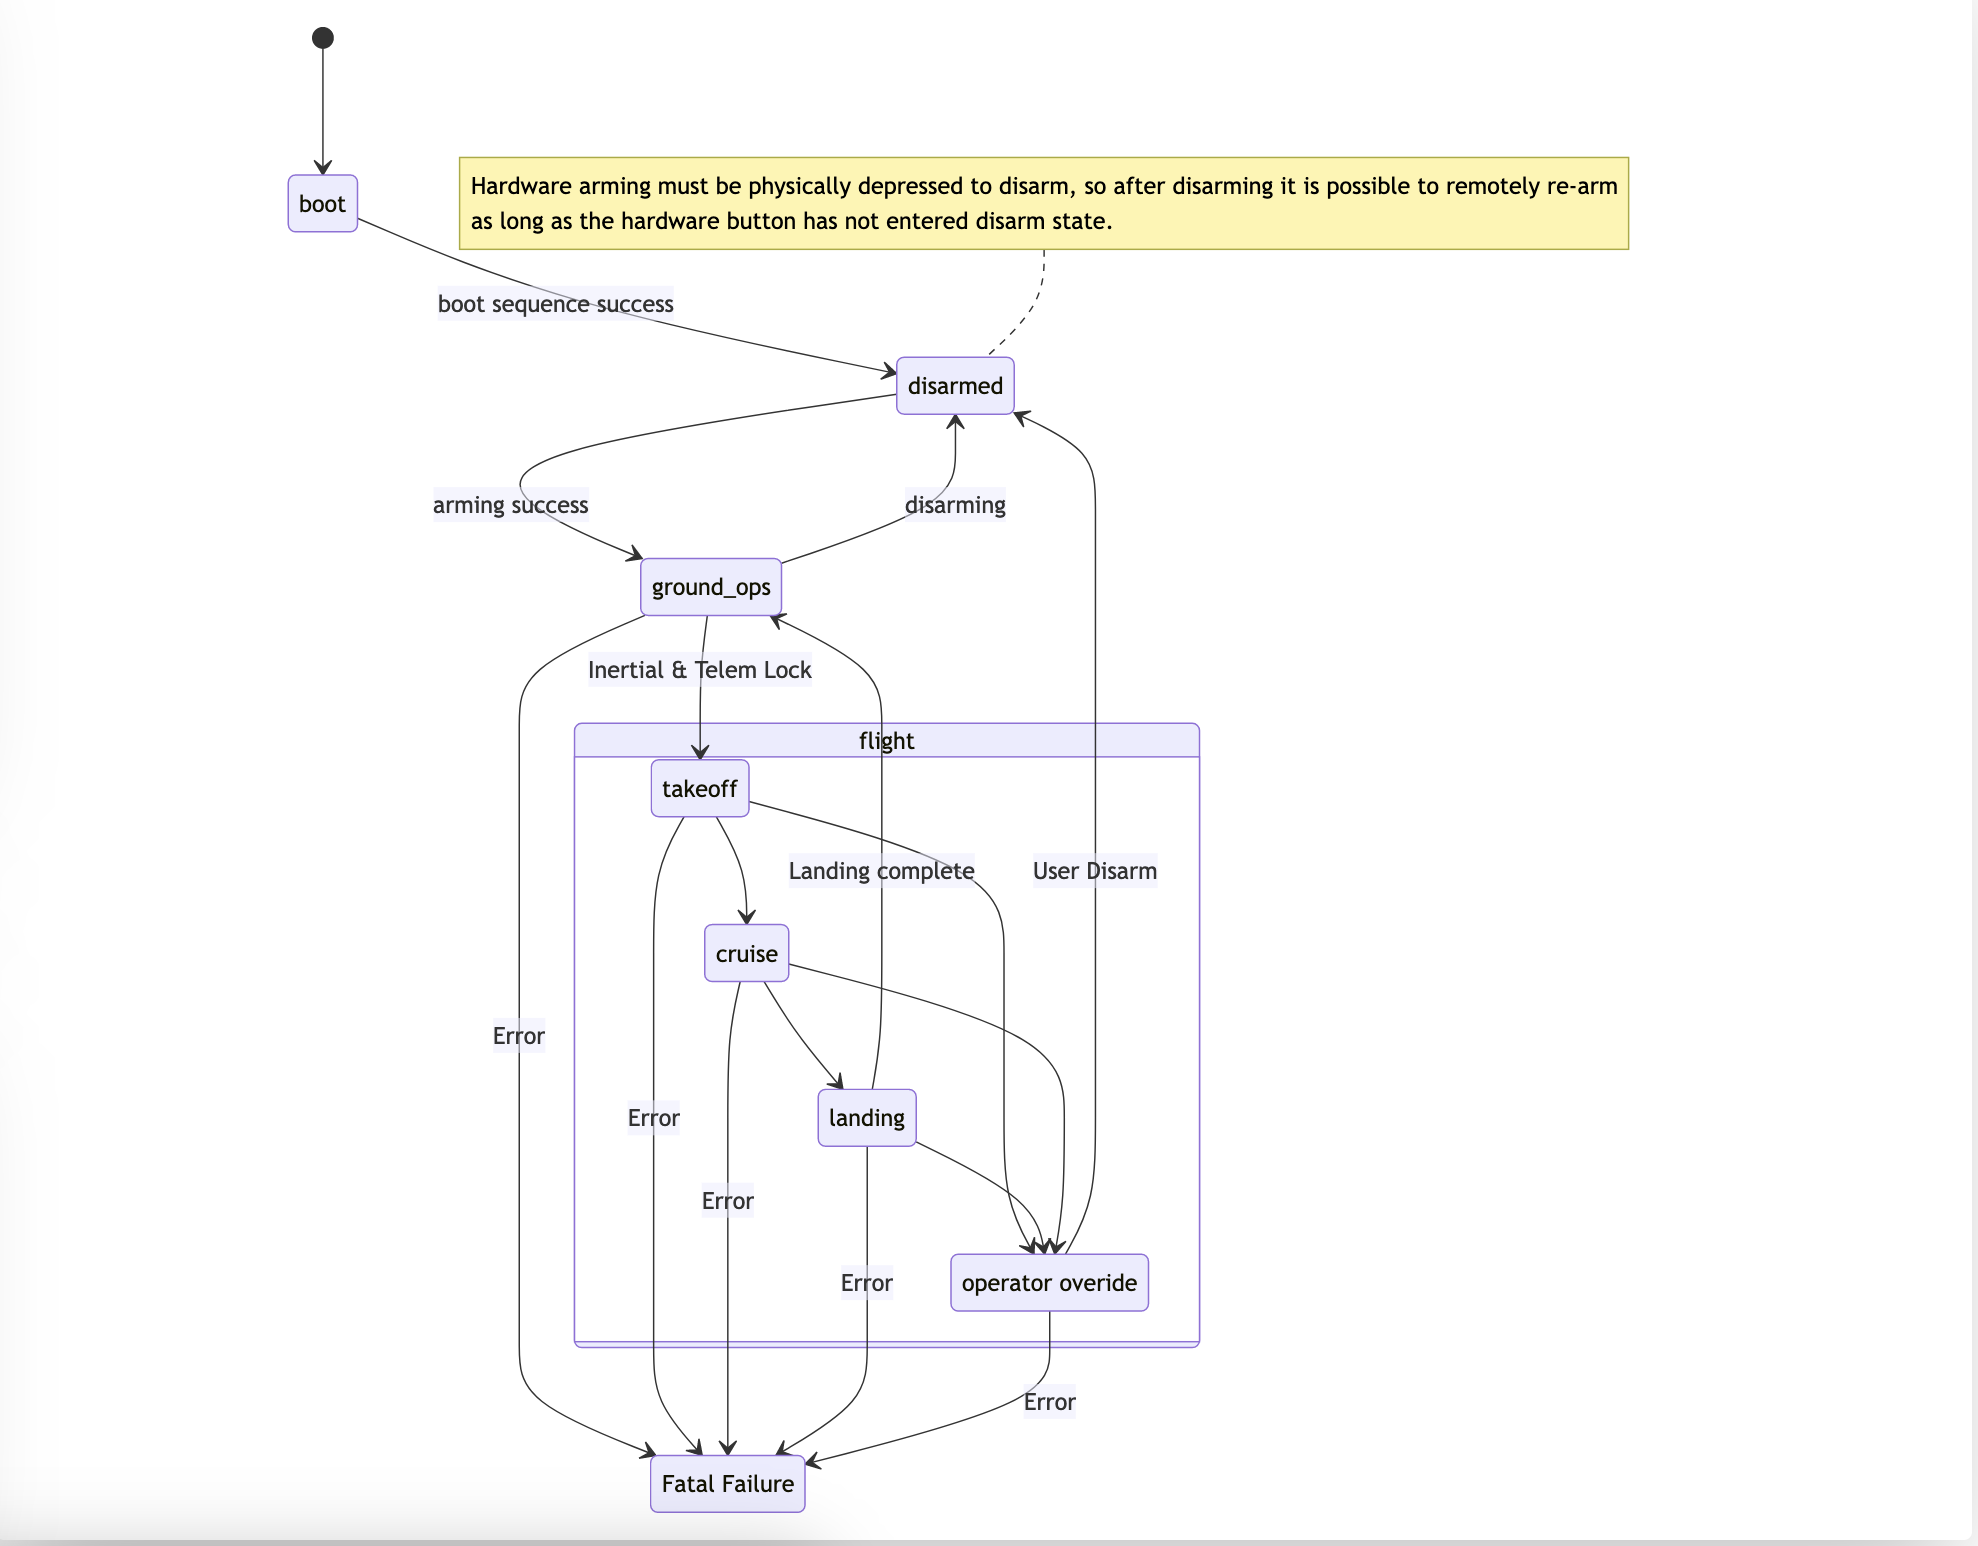
\includegraphics[scale=0.15]{sm-arch}
\end{figure}

\subsubsection{Integrated Monitoring and Command Station}

There are two direct methods of communication between a pilot and the aircraft.
The first is with a traditional radio transmitter manually. In this mode, the
pilot inputs the thrust, yaw, pitch and roll and directly causes the aircraft
to speed up and turn. The second is through the Integrated Monitoring and
Command Station (IMACS), telling the on-board autopilot the desired action to
take (e.g. fly, travel to waypoint, land) and having minimal or no human
interaction thereafter.

\begin{figure}[h]
	\caption{IMACS Setup page for monitoring aircraft attitude and power usage.}
	\centering
	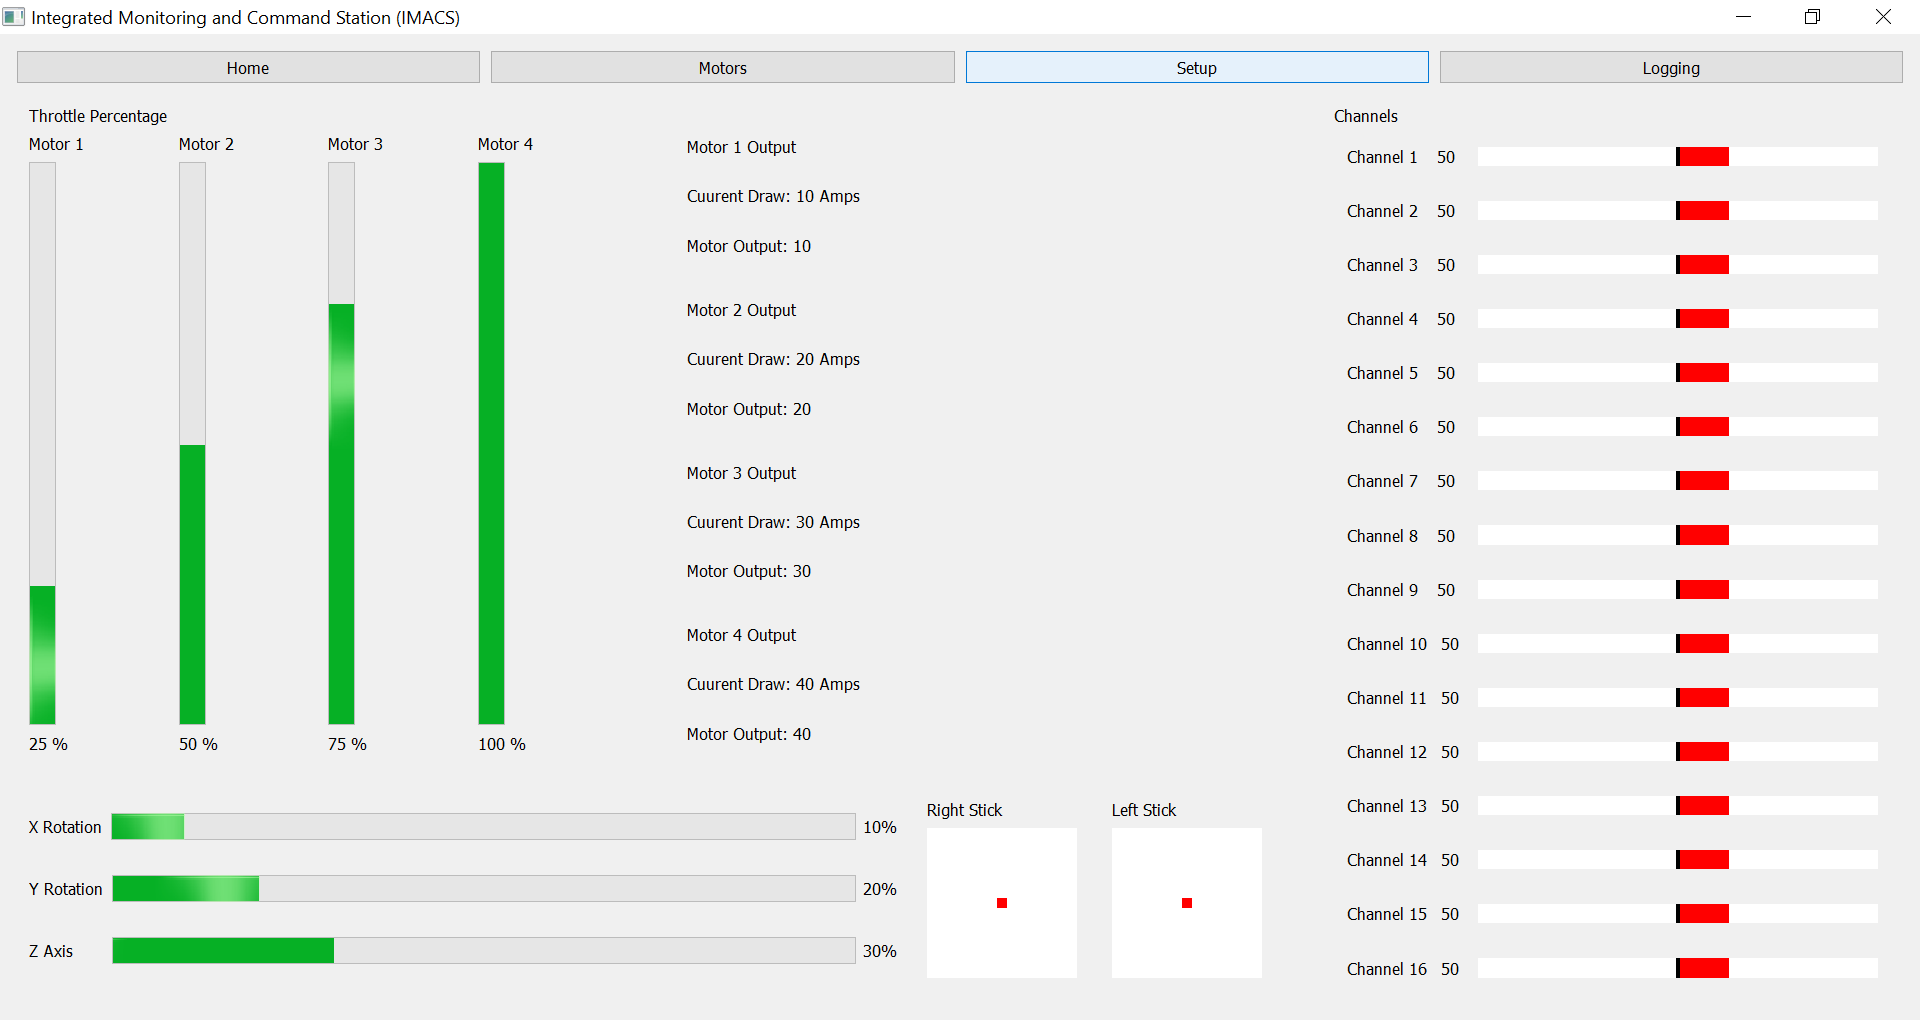
\includegraphics[scale=0.4]{imacs-outputs}
\end{figure}

IMACS is designed to be the primary method of monitoring and communication with
the aircraft. It has a desktop user interface written in Python with QT that
displays various aircraft information and statistics, including the GPS position,
ground and airspeed, battery levels and power usage, altitude, attitude, motor
outputs, and a low-latency video transmission feed.

IMACS also provides an interface for controlling the operation of the aircraft,
such as switching between flight modes (VTOL and fixed-wing), the mandatory
safety kill-switch, waypoint selection and flight path planning, a return-to-home mode, and delegating back to teleoperation and manual flying if necessary.

\begin{figure}[h]
	\caption{IMACS waypoint management interface}
	\centering
	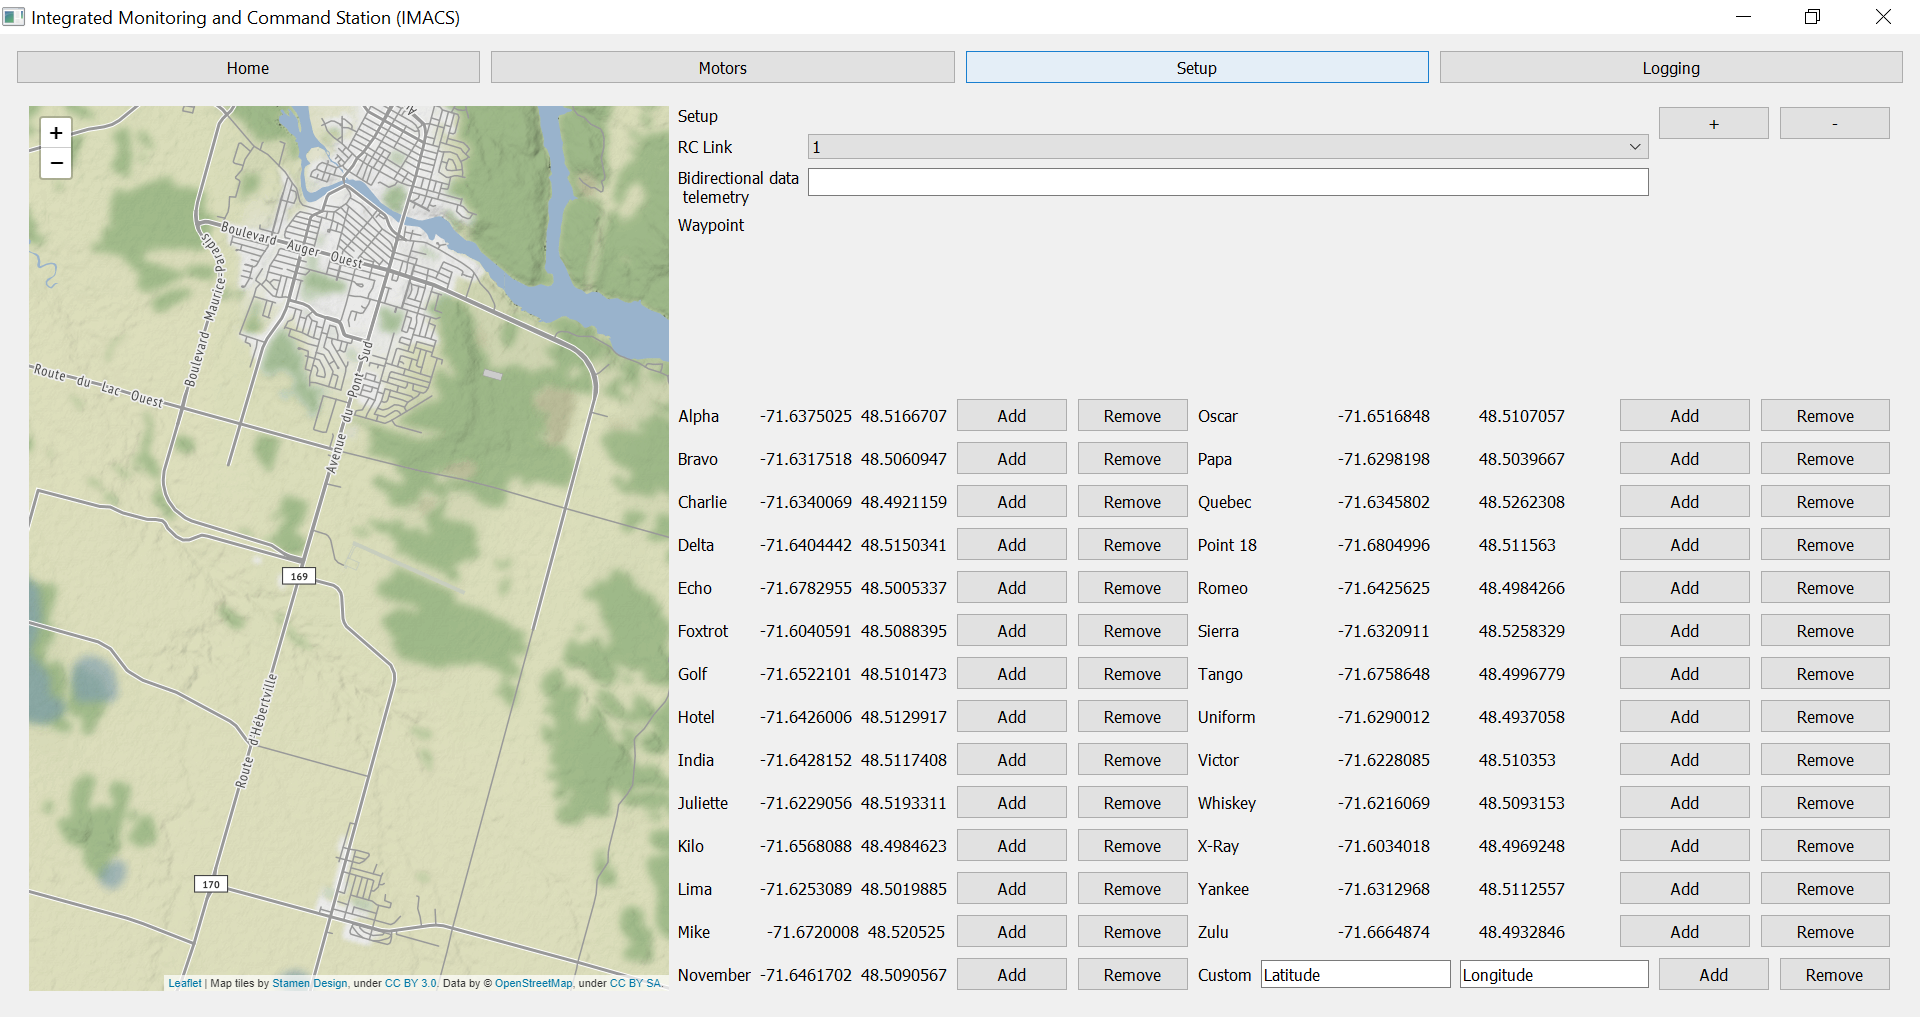
\includegraphics[scale=0.4]{imacs-waypoints}
\end{figure}

The entire IMACS system is designed to be easy to setup and operate in outdoor
conditions and setup up by no more than two people, and integrate with antenna
tracking systems to increase range to the required 5km for the competition.

\subsubsection{Communication Infrastructure}

The primary method of bidirectional communication between the aircraft and
IMACS will happen with the use of RFD 900x modems, one connected to the ground
station and the other to the aircraft. The RFD 900x modems can communicate over
40 km and support serial communication with 2 RP-SMA connectors. They allow for
communication between drone and Ground Station PC similar to a wired serial
connection. 

The flight controllers have support for hardware add-ons. A direct UART
connection is consumed and processed by ZeroPilot to enable communication. On
the ground, the a RFD 900x modem will use a jumper to a USB connection to
interface and communicate with the IMACS.

An antenna tracking system will also be used to improve the data link. On the
ground, a large antenna array will be installed on a tripod with a rotating
platform. Two servos will allow the antenna tracking system to change the pan
and tilt of the antenna to point it directly towards the aircraft.

To autonomously determine the desired pan and tilt of the antenna, a GPS module will also be installed on the tracking antenna. The ground station will provide the GPS coordinates and altitude of the aircraft. An onboard microcontroller on the tracking antenna will use this information to point the antenna precisely at the aircraft.

\begin{figure}[h]
	\caption{Communication between the ground station and the aircraft}
	\centering
	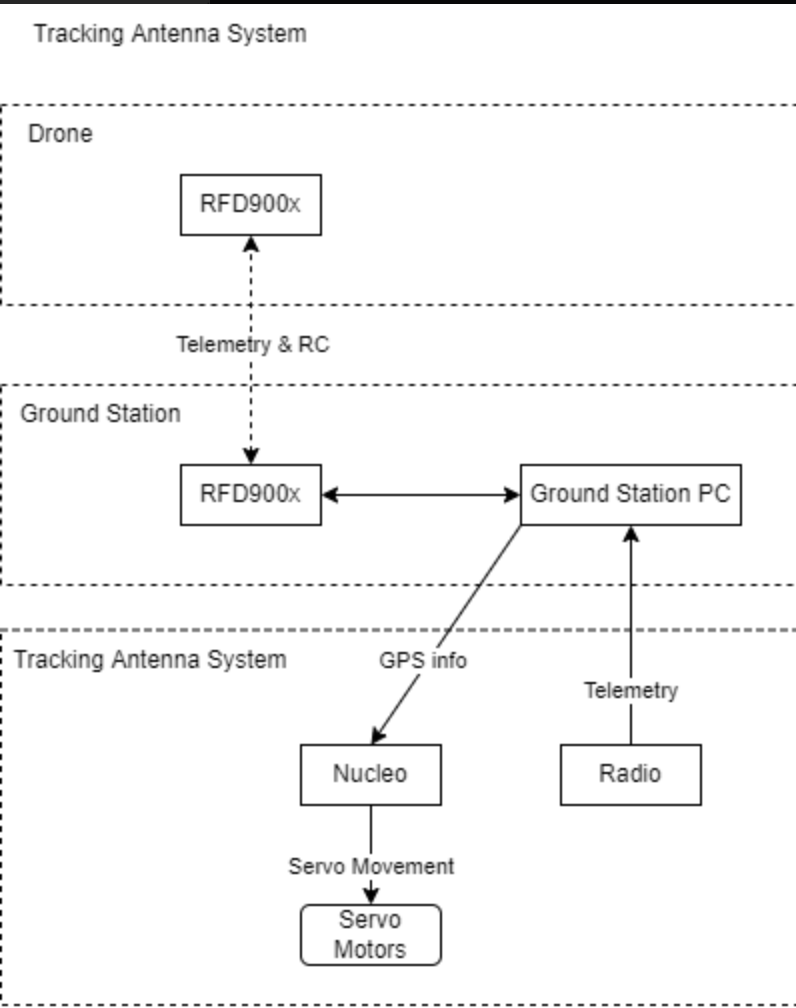
\includegraphics[scale=0.6]{rfd-overview}
\end{figure}

\subsubsection{Airframe Development}

\begin{figure}[h]
	\caption{Airframe ISO view}
	\centering
	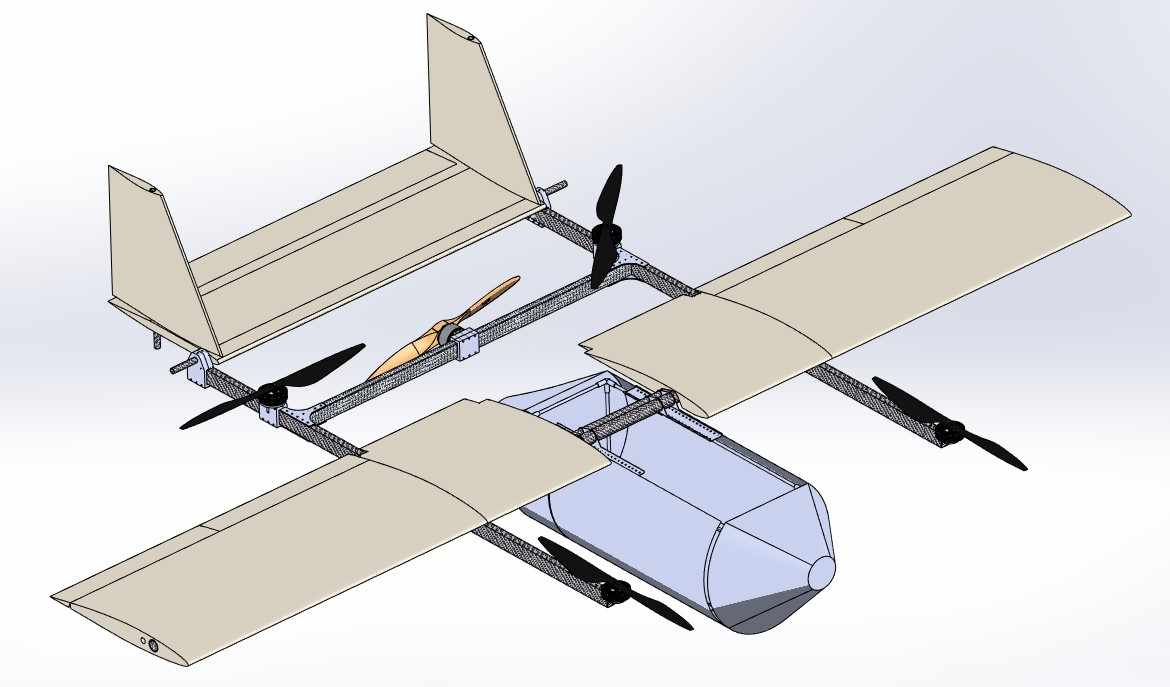
\includegraphics[scale=0.3]{airframe}
\end{figure}

The airframe has been been iterated numerous times in order to minimize weight and manage surface area and drag to compromise for flight characteristics during VTOL and fixed-wing operation.

\todo{Discuss the following talking points}

\begin{itemize}
	\item Sizes and dimensions for the various parts (fuselage, wingspan,
		length, height)
	\item Materials which are being used to construct the aircraft
	\item Aerofoil design and considerations
	\item Weight and thrust calculations, efficiency if considered (drag?)
	\item fuselage design and seats for realism, loading and unloading passengers
\end{itemize}

\subsubsection{VTOL System}

\todo{Discuss the following talking points}

\begin{itemize}
	\item Level of complexity in terms of implementing this from software
	\item Considerations with integrating with flight controller and power
		distribution
	\item (perhaps bring up in alternate solutions): impracticalities for
		having rotating motors for more thrust in fixed-wing
	\item Motor selection for push vs lift
\end{itemize}


%%%%%%%%%%%%%%%%%%%%%%%%%%%%%%%%%%
%
% Automation and CV
%
%%%%%%%%%%%%%%%%%%%%%%%%%%%%%%%%%%

\subsection{Automation and CV}


\subsubsection{Autonomous Flight}

\todo{Discuss the following talking points}

\begin{itemize}
	\item PID tuning rig and teaching the aircraft to fly
	\item How do we convert waypoint information into flight control operations?
	\item Sensor fusion implementation and interfacing with LOS
\end{itemize}

\subsubsection{Path Planning and Optimization}

\todo{Discuss the following talking points}

\begin{itemize}
	\item Using dijkstra's algorithm?
	\item reinforcement learning algorithms to 
	\item can be precomputed before hand
	\item Any other details for development and integration of software
\end{itemize}

\subsubsection{Autonomous Landing Capabilities}

\todo{Discuss the following talking points}

\begin{itemize}
	\item Already have approximate location for landing pad from coordinates
	\item using downward facing camera 
	\item Discussion implementation and usage of the Jetson to improve performance
		and run our CV system
\end{itemize}

\begin{figure}[h]
	\caption{Autonomous landing architecture diagram}
	\centering
	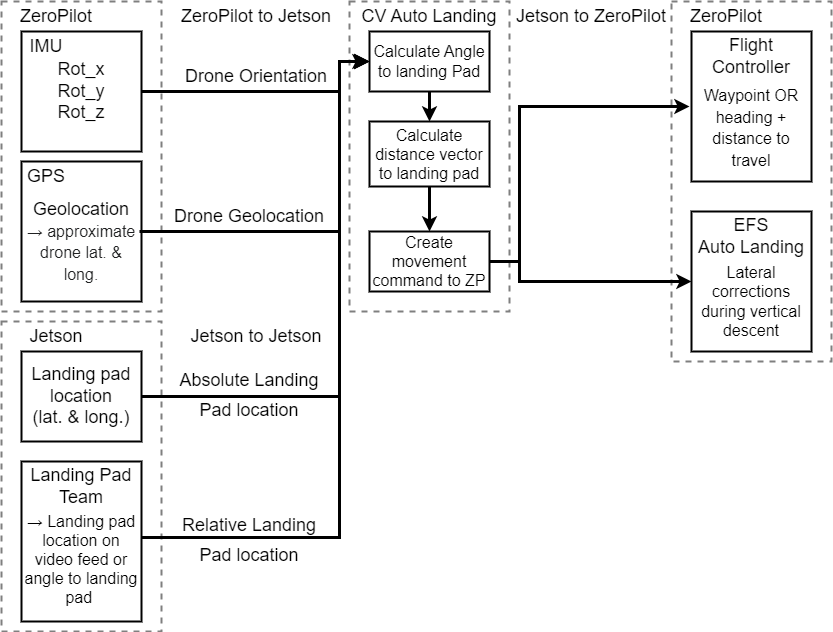
\includegraphics[scale=0.3]{autonomous-landing}
\end{figure}

\subsection{Passenger Safety Considerations}

\subsubsection{Enclosed and protected passenger seating}

All passengers within the aircraft are fully enclosed within the carbon fiber
fuselage and have individual seatbelts to keep them securely fastened during
the flight. All passengers, seats, and other objects within the fuselage are
secured and will not shift. Furthermore, The primary hatch on the side of the
aircraft is easily accessed and can be used to disembark from the aircraft in
case of emergencies.

Furthermore, in case of an electric failure with the aircraft systems (such as the battery), the fuselage of the aircraft is sufficiently protected in order to keep the passengers safe from any potential risk of fire or smoke.

\subsubsection{Software and Hardware redundant components}

\todo{Include any redundant software and hardware features we might have. This
might include having multiple GPS components, backup flight controller w/
ArduPilot in case of failure with ZeroPilot, and any potential failsafe mode.
Also might be good to talk about how we deal with RC link loss (10 seconds
before flight termination)}

\subsubsection{Motor and Speed Controller Failure}

Due to the aerodynmic nature of the aircraft, in situations where the aircraft suffers motor or an electronic speed controller failure, the aircraft will have the opportunity to switch to the other flight mode to reduce the risk of a crash. During cruise, the failure of the push propeller will provide the aircraft enough gliding time to attempt troubleshooting the issue and transition into VTOL mode to perform an emergency landing.

During VTOL, the window to troubleshoot and recover from failure will be shorter, however, there still is the opportunity to attempt to recover into fixed-wing mode and perform a traditional fixed-wing emergency landing.
